\documentclass[aspectratio=169]{beamer}
\usetheme{Madrid}
\usecolortheme{beaver}
\usepackage[utf8]{inputenc}
\usepackage[T1]{fontenc}
\usepackage{tikz}
\usepackage{amssymb}
\usepackage{graphicx}
\setbeamertemplate{navigation symbols}{}
\setbeamercolor{title}{fg=white,bg=cyan!60!black}
\setbeamercolor{frametitle}{fg=white,bg=cyan!50!black}
\setbeamercolor{block title}{bg=cyan!15,fg=black}
\setbeamercolor{block body}{bg=cyan!5,fg=black}

\title{Story Studio 5 — Choose a Path}
\subtitle{Lesson 1: Two Endings}
\author{ByteForge --- Grade 7 --- Game Maker}
\date{}

\begin{document}

\begin{frame}
    \titlepage
\end{frame}

\begin{frame}{A variable is only useful if something CHECKS it}
    \Large
    A variable stores a choice; IF/ELSE is what actually MAKES that choice matter — without a branch, every choice would look the same.

    \begin{center}
    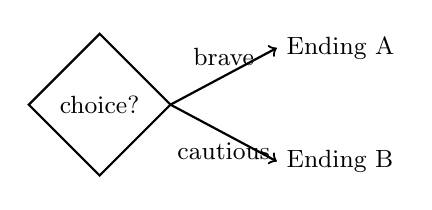
\begin{tikzpicture}[scale=0.9]

        \draw[thick] (1,1) -- (2,0) -- (1,-1) -- (0,0) -- cycle;
        \node at (1,0) {\small choice?};
        \draw[->, thick] (2,0) -- (3.5,0.8) node[midway, above] {\small brave};
        \draw[->, thick] (2,0) -- (3.5,-0.8) node[midway, below] {\small cautious};
        \node[right] at (3.5,0.8) {\small Ending A};
        \node[right] at (3.5,-0.8) {\small Ending B};
    \end{tikzpicture}
    \end{center}
\end{frame}

\begin{frame}{Your Turn}
    \Large
    Open the student map, find \textbf{Story Studio 5 — Choose a Path}, and complete
    the \textbf{Two Endings} challenge --- everything you just saw, they now do themselves.
\end{frame}

\end{document}
